\documentclass[a4paper,openany]{uantwerpenassignment}

\usepackage[dutch]{babel}
\usepackage{titlesec}
\usepackage{tikz}
\usepackage{pythonhighlight}
\usepackage{amsmath}
\usepackage{array}
\usepackage{subcaption}
\usepackage{listings}\usepackage[nottoc,numbib]{tocbibind}

\renewcommand{\lstlistingname}{Code}

\newenvironment{conditions}
  {\par\vspace{\abovedisplayskip}\noindent\begin{tabular}{>{$}l<{$} @{${}={}$} l}}
  {\end{tabular}\par\vspace{\belowdisplayskip}}

\definecolor{code}{HTML}{ecf0f1}
\definecolor{codetext}{HTML}{d9534f}
\newcommand{\codeword}[1]{
    \colorbox{code}{\texttt{\textcolor{codetext}{#1}}}
}

\newcommand{\reference}[1]{\textit{\ref{#1}. \nameref{#1}}}
\newcommand{\figref}[1]{\textit{Figuur \ref{#1}}}
\newcommand{\coderef}[1]{\textit{Code \ref{#1}}}
\newcommand{\ts}{\textsuperscript}

\facultyacronym{TI}

\title{\sffamily Chess AI-Agent}
\subtitle{\sffamily5-Artificiële Intelligentie}
\author{\sffamily Mathias Maes, Tijs Van Alphen \\en Willem Van der Elst}

\programme{BA}{IW}{EI}

\academicyear{2020-2021}

\publisher{}

\titleformat{\chapter}{\sffamily\huge\bfseries}{\thechapter.}{10pt}{\sffamily\huge\bfseries}
\titleformat{\section}{\sffamily\LARGE\bfseries}{\thesection.}{10pt}{\sffamily\LARGE\bfseries}
\titleformat{\subsection}{\sffamily\Large\bfseries}{\thesubsection.}{10pt}{\sffamily\Large\bfseries}
\titleformat{\subsubsection}{}{}{10pt}{\sffamily\large\bfseries}


\begin{document}

\sffamily
\maketitle

\tableofcontents

\chapter{Keuze}
\label{keuze}

Het type AI was een belangrijke keuze van dit project. Het moest haalbaar zijn om te implementeren binnen de beperkte tijdsperiode en we moesten onze eigen niet-supercomputers gebruiken om te treinen. Een lijst  met de voor- en nadelen van de verschillende opties werd opgesteld.\\[2 \baselineskip]


\textbf{Search}:\\
Er zijn te veel mogelijke states ($\approx10^{120}$) om de hele tree uit te werken. 

\textbf{Multi-Agent search} (Minimax, Alpha-Beta pruning):\\
Deze methode wordt gebruikt door meerdere bronnen, maar we hebben er nog geen ervaring mee. 

\textbf{Reinforcement learning} (Generalised Q learning):\\
We hebben dit al gebruikt en daarom begrijpen we het al en kunnen we het snel implementeren.\\
Eenmaal getraind, zal het optimaal functioneren. De training heeft echter veel tijd nodig en de keuze van de features is niet zo voor de hand liggend.

\textbf{Neural network/ Deep learning:}
Onze ervaring met Deep learning is nogal beperkt. We weten niet goed wat we als in- en output moeten nemen. \\[2 \baselineskip]


Q-Learning leek ons het interessantst, maar Minimax is haalbaarder en zou sowieso een goed resultaat leveren. Uiteindelijk besloten we om beide methodes uit te werken. We hadden namelijk een thesis\cite{rl} gevonden die een minimax agent gebruikte als feature voor een generalized Q-Learner.

\chapter{Alpha-Beta Pruning}

\section{Utility}
\label{utility}

Onze utility is grotendeels gebaseerd op de rewards van onze Q-Learner die later in dit verslag behandelt worden.
Op dit moment volstaat het om een simpele versie van onze utility te aanschouwen:


$$
u(S) = 
\begin{cases}
 100 &\mbox{Schaakmat gewonnen}\\
    -30 &\mbox{Gelijkspel of Stalemate}\\
    -100 &\mbox{Schaakmat verloren}\\
    c + C + \Delta M + \Delta m + s + f_q &\mbox{Bij overige situaties}
\end{cases}
$$

\begin{conditions}
    c & Of er gecastled is met de vorige move\\
    C & Of het bord in schaak staat\\
    \Delta M & Het materiaal verschil op het bord\\
    \Delta m & Het verschil in mobility\\
    s & De positie score voor alle eigen stukken\\
    f_q & Een gewogen(geleerd of niet-geleerd) aantal features
\end{conditions}

Deze kleine sub-functies worden later nog besproken in \reference{features}.

\chapter{Q-Learning Agent}

\section{Generalization}

De eerste agent die we maakten, was de Q-agent. Deze is generalized omdat, zoals besproken in \reference{keuze}, het praktisch onmogelijk is om elke staat te bezoeken. Daarom dat we niet 'gewoon' Q-learning kunnen gebruiken, maar wel generalized Q-learning.

\section{Features}
\label{features}

We hebben een hoop features gedefinieerd. Deze zijn voornamelijk gebaseerd op features uit de paper\cite{rl}. De bedoeling van deze features is om een state zo goed mogelijk te definiëren. Je kan hieronder een beschrijving vinden van elks van onze 55 features.

We berekenen onze features als volt:

$$
Q(s,a) = \sum_{i} w_{i} \cdot \sigma \left( f_i(s, a)\right)
$$

De $\sigma(x)$ die we in de berekening zien wordt als volgt gedefinieerd:

$$
\sigma(x) = \frac{2}{1 + e^{-x}} - 1
$$

Dit is een aangepaste versie van de bekende sigmoid\cite{WSF} functie. Onze versie zorgt in tegenstelling tot de originele er voor dat waardes in het interval $\left]-1,1\right[$ vallen.\\
Hier zie je de grafiek van de functie:

\begin{figure}[h]
    \centering
    \begin{tikzpicture}[scale=2]
        \draw[->] (-2, 0) -- (2, 0) node[right] {$x$};
        \draw[->] (0, -1.2) -- (0, 1.2) node[above] {$y$};

        \draw[dashed] (-2, 0.5) -- (2, 0.5);
        \node (A) at (-2, 0.6) {\tiny $1$};

        \draw[dashed] (-2, -0.5) -- (2, -0.5);
        \node (B) at (-2, -0.6) {\tiny $-1$};

        \draw[scale=0.5, domain=-3.9:3.9, smooth, variable=\x, blue] plot ({\x}, { 2/(1 + exp(-\x)) - 1 });
        \node[blue] (C) at (0.4, 0.32) {$\sigma$};
    \end{tikzpicture}
    \caption{$\sigma(x)$} \label{fig:sigmoid}
\end{figure}



\subsection{Amount of Pieces}
Een andere feature die we gebruiken is het aantal soort stukken van elke speler. We doen dit 1 keer voor alle schaakstukken van het bord, zowel de onze als die van de tegenspeler.

We creëerden ook voor elke type schaakstuk 2 features. Eén die bijhoud hoeveel van dit type schaakstukken je zelf op het bord bevindt en één die bijhield hoeveel je opponent er heeft. Op deze manier zal onze Q-agent leren dat een slecht ding is als de opponent veel stukken van een type en dat het goed is als je zelf veel schaakstukken bezit.

Het laatste wat we ook nakijken is de feature \codeword{AmountBalancePieces()} deze zal de material value van alle stukken van de speler berekenen en de material value van de tegenspeler er af trekken. Wanneer dit getal dus negatief is betekend dat dat de tegenspeler globaal bekeken er beter voor staat als jezelf.


\subsubsection{Material value}
Elk soort schaakstuk krijgt een cijfer dat zijn waarde bepaalt. Zo krijgt de koningin een hogere waarde dan een pion, omdat de koningin belangrijker is. In \coderef{code:material} staat de implementatie van hoe de schaakstukken zich verhouden t.o.v. elkaar.

\begin{lstlisting}[style=mypython,caption={Material Function},captionpos=b,label={code:material}]
def getMaterialValue(piece_type):
    if piece_type is chess.PAWN:
        return 1
    elif piece_type is chess.KNIGHT or piece_type is chess.BISHOP:
        return 3
    elif piece_type is chess.ROOK:
        return 5
    elif piece_type is chess.QUEEN:
        return 9
    elif piece_type is chess.KING:
        return 10

    return 0
\end{lstlisting}

\subsection{Mobility}
De \codeword{Mobility.py} file berekent voor elke type schaakstuk hoeveel vakjes het stuk kan bereiken. 

Dit wordt gebruikt voor de mobility features. Hierbij gaan we voor elke type schaakstuk kijken op hoeveel vakjes die kan terechtkomen. Dit zullen we ook weer doen voor zowel de speler als de tegenspeler.

De feature \codeword{MobilityRookS()} zal voor elke Rook (toren) van de eigen speler (S in de functie staat voor self) berekenen op hoeveel vakjes die kan komen en bij elkaar optellen.

Voor het berekenen van de vakjes gaan kijken of een een legal move zou zijn als we dat stuk naar een vakje zouden zetten, wanneer dit een false teruggeeft betekend het dat we niet naar dat vakje kunnen omdat er al een ander van je schaakstukken op staat. Hier hebben we wat problemen ondervonden voor de opponent omdat we enkel onze eigen stukken kunnen verplaatsen. Onze oplossing hiervoor was een copy van het bord maken gevolgd door een board turn, op deze manier speel je dan zogezegd even als de opponent op het gekopieerde bord. 
\pagebreak

\pagebreak

\subsection{Attackers}
Deze attacked features laten weten hoeveel van je schaakstukken van een bepaald type kunnen worden aangevallen door schaakstukken van de opponent met een inferieure waarde. 

Zo zal bijvoorbeeld de \codeword{AttackedRooksS()} feature calculeren hoeveel van zijn torens kunnen worden aangevallen door een schaakstuk van de tegenspeler met een inferieure waarden, in dit geval de pion, paard of loper.

Voor de opponent te berekenen hebben we het probleem zoals bij moblility op dezelfde manier opgelost.

\subsection{Forks}

De volgende twee features hebben ook zowel voor de speler als de tegenspeler geïmplementeerd.

\subsubsection{Pawn Fork}
Pawn fork gaat kijken hoeveel van jouw pionen 2 superieure stukken van de tegenstander kan pakken.

In \figref{fig:pawnFork} zal pion op d4 meetellen bij de pawn fork som, omdat deze 2 schaakstukken met een hogere material value kan nemen. Terwijl pion op g4 niet zal worden meegeteld.

\subsubsection{Knight Fork}
Gelijkend aan de Pawn fork zal de Knight fork ook kijken welke van je paarden 2 superieure schaakstukken van de tegenspeler kan nemen.

In \figref{fig:knightFork} zal het paard op d5 worden meegeteld, maar het paard op g2 niet. Het paard op g2 wordt niet meegeteld omdat het paard dat deze kan nemen niet superieur is t.o.v. zichzelf.


\begin{figure}[h]
    \centering
    \begin{subfigure}{.4\textwidth}
        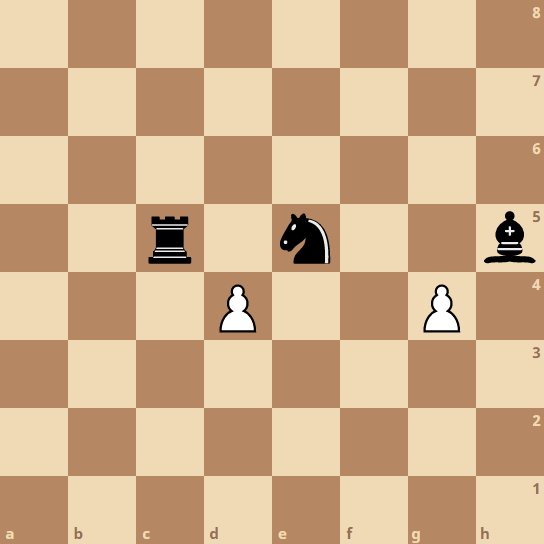
\includegraphics[width=170pt]{images/pawnFork.png}
        \caption{Example of pawn fork}
        \label{fig:pawnFork}
    \end{subfigure}
    \begin{subfigure}{.4\textwidth}
        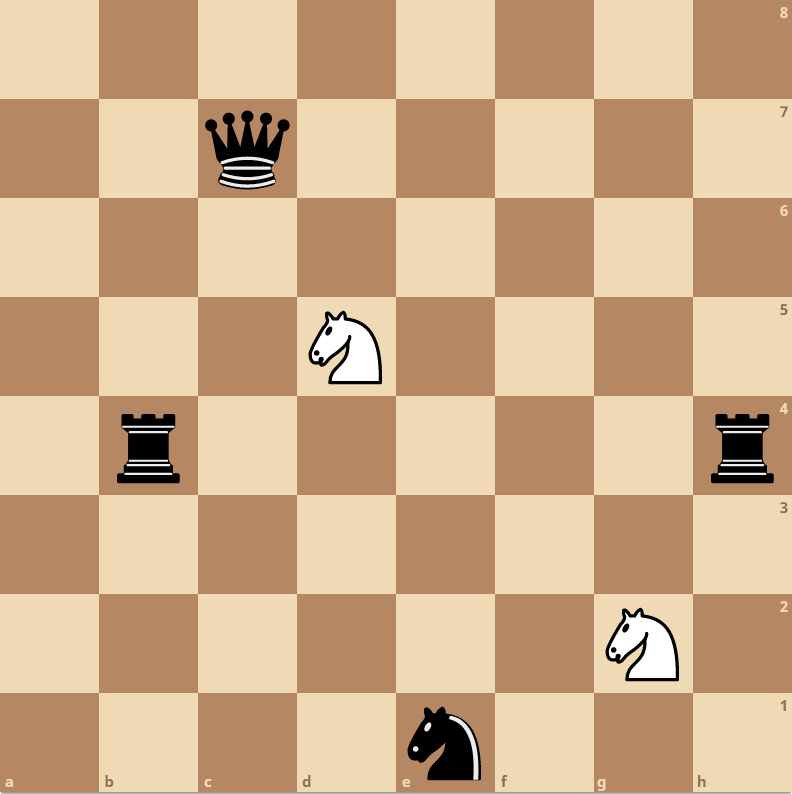
\includegraphics[width=170pt]{images/knightFork.png}
        \caption{Example of knight fork}
        \label{fig:knightFork}
    \end{subfigure}
    \caption{Examples of forks}
\end{figure}

\subsection{Control}
\subsubsection{Center Control}
Center control is een feature die ons verteld hoeveel pawn je hebt staan op de vakjes D4, E4, D5, E5. Deze 4 vakjes zijn het belangrijkste van het bord, omdat deze vakjes het grootste trafiek hebben van het bord.

Deze feature wordt ook weer voor zowel de eigen speler als de tegenspeler gecreëerd.

\subsubsection{Board Control}

\subsection{connectivity}
\subsection{provokers}
\subsection{position score}
\subsection{Rooks on 7th rank}
Deze feature gaat kijken hoeveel torens er van de speler op de zevende rang staan. Hierbij wordt er geteld vanaf de kant van de speler zelf. Dus de tegenspeler zal dat dus rij 2 zijn. Wanneer er torens op de 7\ts{de} rang staat sta je heel sterk in het spel. Dit komt doordat je de bewegingsruimte van de opponent zijn koning sterk wordt beperkt en dat alle andere stukken op die rank niet veilig staan.

\begin{figure}[h]
    \centering
    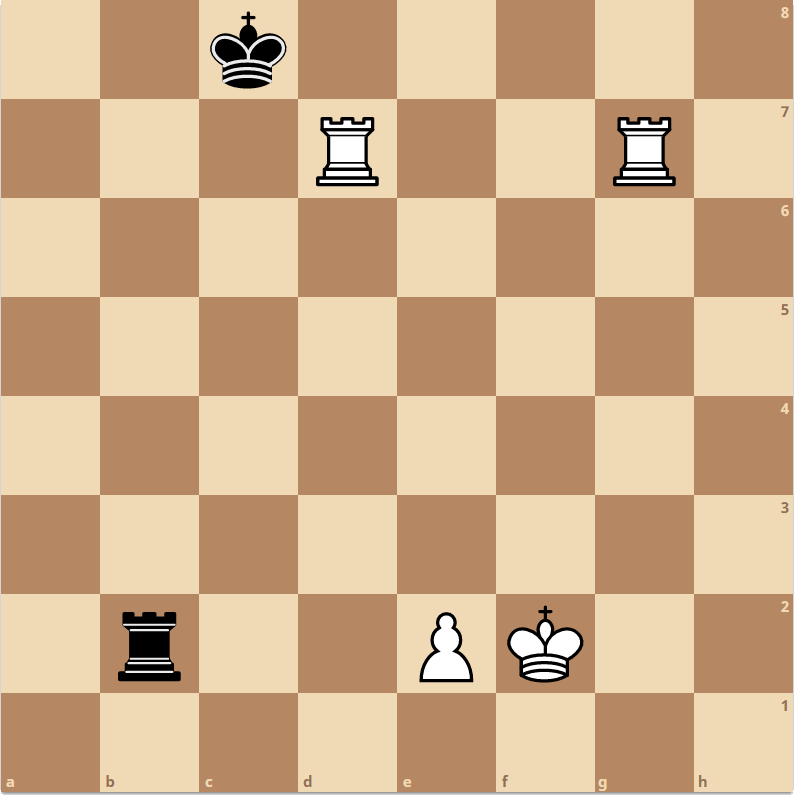
\includegraphics[width=170pt]{images/rooks7rank.png}
    \caption{Example of rooks on 7\ts{th} rank}
    \label{fig:rooks7rank}
\end{figure}


\subsection{king distance to center}
\subsection{Castling}

Dit is een vrij eenvoudige feature die kijkt of de agent gecastled heeft. In \figref{fig:castling2} en \figref{fig:castling3} staan 2 voorbeelden afgebeeld van castling.

\begin{figure}[h]
    \centering
    \begin{subfigure}{.3\textwidth}
        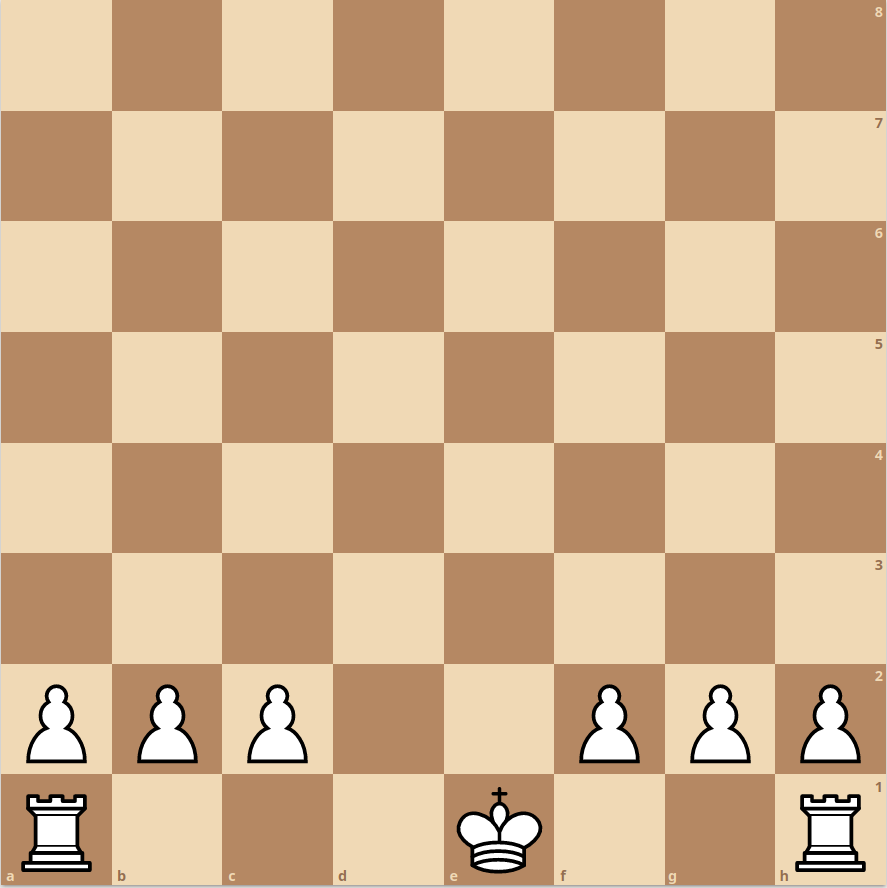
\includegraphics[width=130pt]{images/castling1.png}
        \caption{Initial state}
        \label{fig:castling1}
    \end{subfigure}
    \begin{subfigure}{.3\textwidth}
        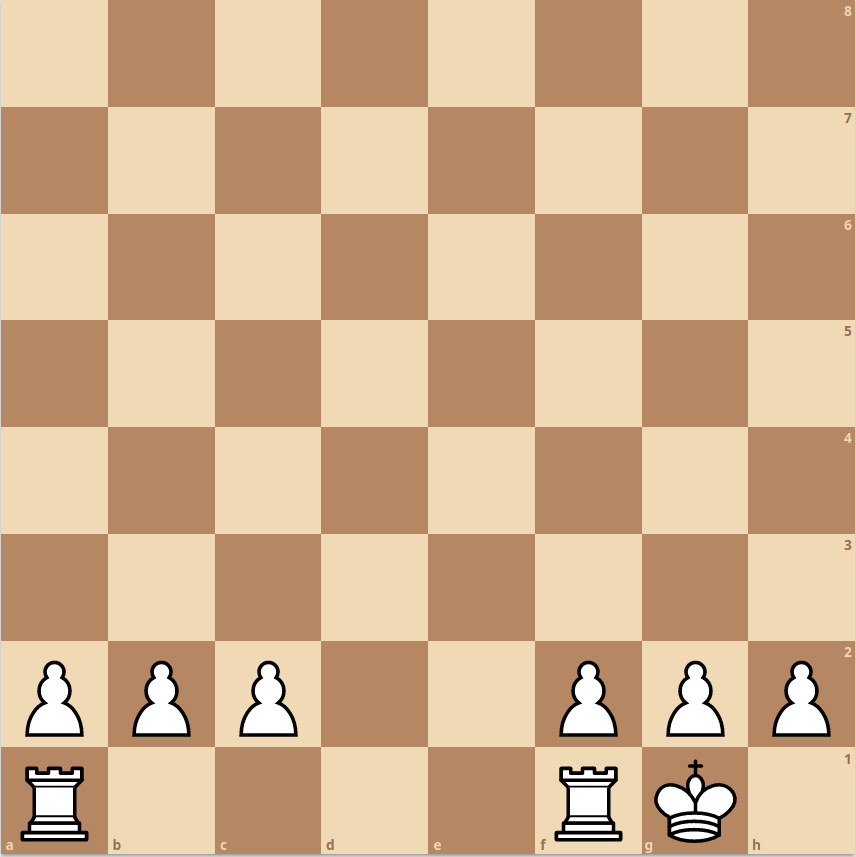
\includegraphics[width=130pt]{images/castling2.png}
        \caption{Short castling}
        \label{fig:castling2}
    \end{subfigure}
    \begin{subfigure}{.3\textwidth}
        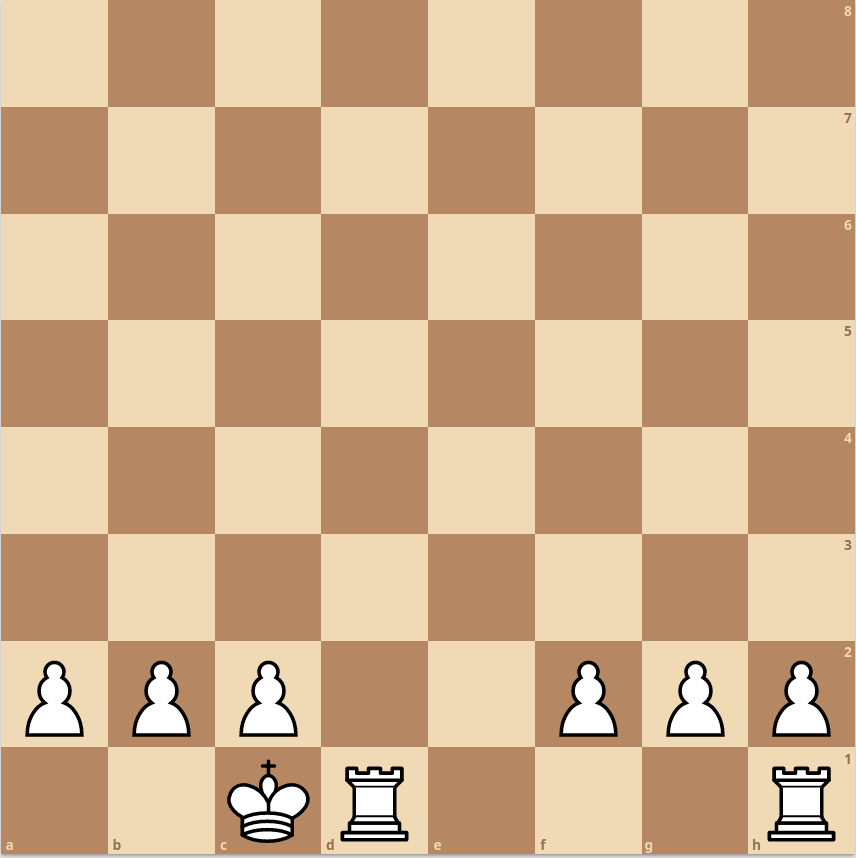
\includegraphics[width=130pt]{images/castling3.png}
        \caption{Long castling}
        \label{fig:castling3}
    \end{subfigure}
    \caption{Examples of castling}
    \label{fig:castling}
\end{figure}

\subsection{double pawns}
\subsection{light pieces on }


\subsection{Alpha-beta Agent prediction feature}

Deze feature laat een onze alpha-beta agent een keuze maken in de huidige situatie. Als deze keuze overeenkomt met de keuze van de Q-agent dan returned deze feature $1$ zo niet dan krijgen we een return waarde van $0$. Deze feature kent ook optimalisaties maar hierover later meer in \reference{caching}.




\section{Reward}

De reward functie is als volgt gedefinieerd:


$$
R(S, a, NS) = 
\begin{cases}
    100 &\mbox{Schaakmat gewonnen}\\
    -30 &\mbox{Gelijkspel of Stalemate}\\
    -100 &\mbox{Schaakmat verloren}\\
     C_O(S, a) - C_S(NS) + c(S) + \Delta M &\mbox{Bij overige situaties}
\end{cases}
$$

\begin{conditions}
    C_O & of de opponent in schaak staat\\
    C_S & of de agent in schaak staat\\
    c &   of er gecastled is\\
    \Delta M & het materiaal verschil op het bord
\end{conditions}


\chapter{Optimalisaties}

We hebben een hoop optimalisaties moeten toevoegen aan onze Q-Learner om hem zo rap mogelijk te laten denken.

\section{Multi-Threading}

We hebben multi-threading toegevoegd aan onze q-learner zo berekent hij de q-waarde van elke actie in een aparte thread. We hebben bewust niet gekozen om elke feature apart omdat dit onze timing issues verergerde in plaat van verbeterde. We hebben door multi-threading onze iteratie tijd met $20\%$ weten dalen.

In \figref{fig:singlethreaded} en \figref{fig:multithreaded} is het verschil te zien tussen single-threaded \tiny(\ref{fig:singlethreaded})\small{ }en multi-threaded \tiny(\ref{fig:multithreaded})\small{ }CPU usage.

\begin{figure}[h]
    \centering
    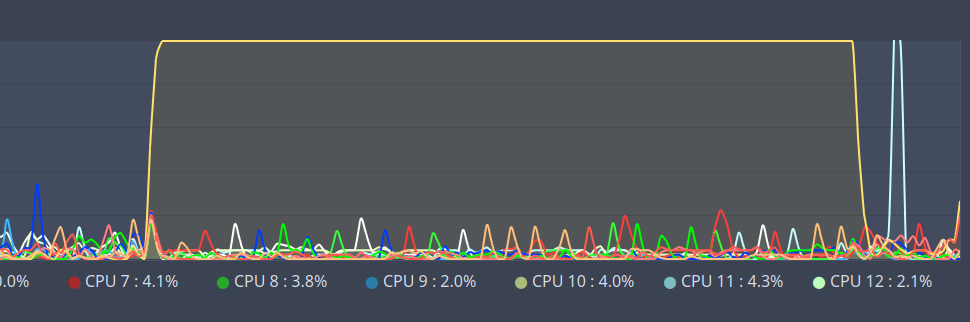
\includegraphics[width=300pt]{images/singlethreaded.png}
    \caption{Single Threaded Q-Learner CPU usage}
    \label{fig:singlethreaded}
\end{figure}

\begin{figure}[h]
    \centering
    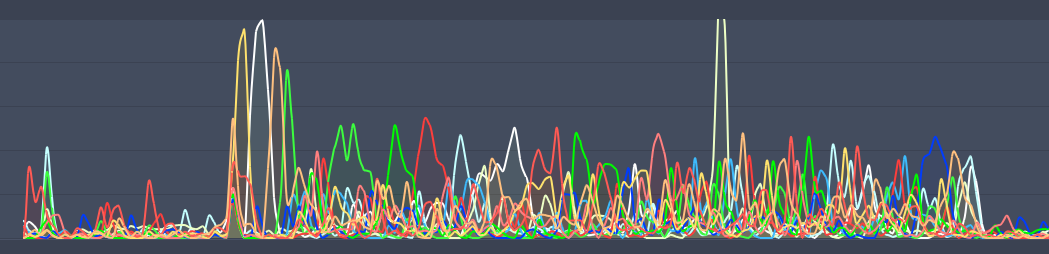
\includegraphics[width=350pt]{images/multithreaded.png}
    \caption{Multi Threaded Q-Learner CPU usage}
    \label{fig:multithreaded}
\end{figure}

\section{Caching}
\label{caching}

We gebruiken ook veel plaatsen caching zodat we niet 2 keer hetzelfde moeten uitrekenen. De meest bijzondere cache is deze voor onze alpha-beta feature, deze moet per bord state maar 1 keer uitvoeren waardoor we de alpha-beta langer kunnen laten zoeken en een hoop tijd besparen.
Det tijd die we hierdoor besparen per iteratie kan soms tot een minuut of 2 oplopen.

Dit was uiteraard wel een trade off met memory usage, echter werd de extra gebruikte memory overschaduwd door de tijdswinsten.

\chapter{Resultaten}

Hier vind je al onze resultaten van het uitbundig trainen. We hebben deze in de loop van 5 dagen op een cloud server laten trainen. 1 dag tegen stockfish en de overige 4 dagen tegen onze alpha-beta agent.

Je kan ook altijd onderaan de commando's vinden die we gebruikt hebben bij het trainen van onze agent.

\section{GrandQ vs. Stockfish (0-544)}

In de eerste leer sessie hebben we onze Q-agent tegen stockfish laten trainen zoals verwacht heeft onze agent nooit kunnen winnen, maar heeft wel hieruit nuttige info kunnen leren.

\begin{figure}[h]
    \centering
    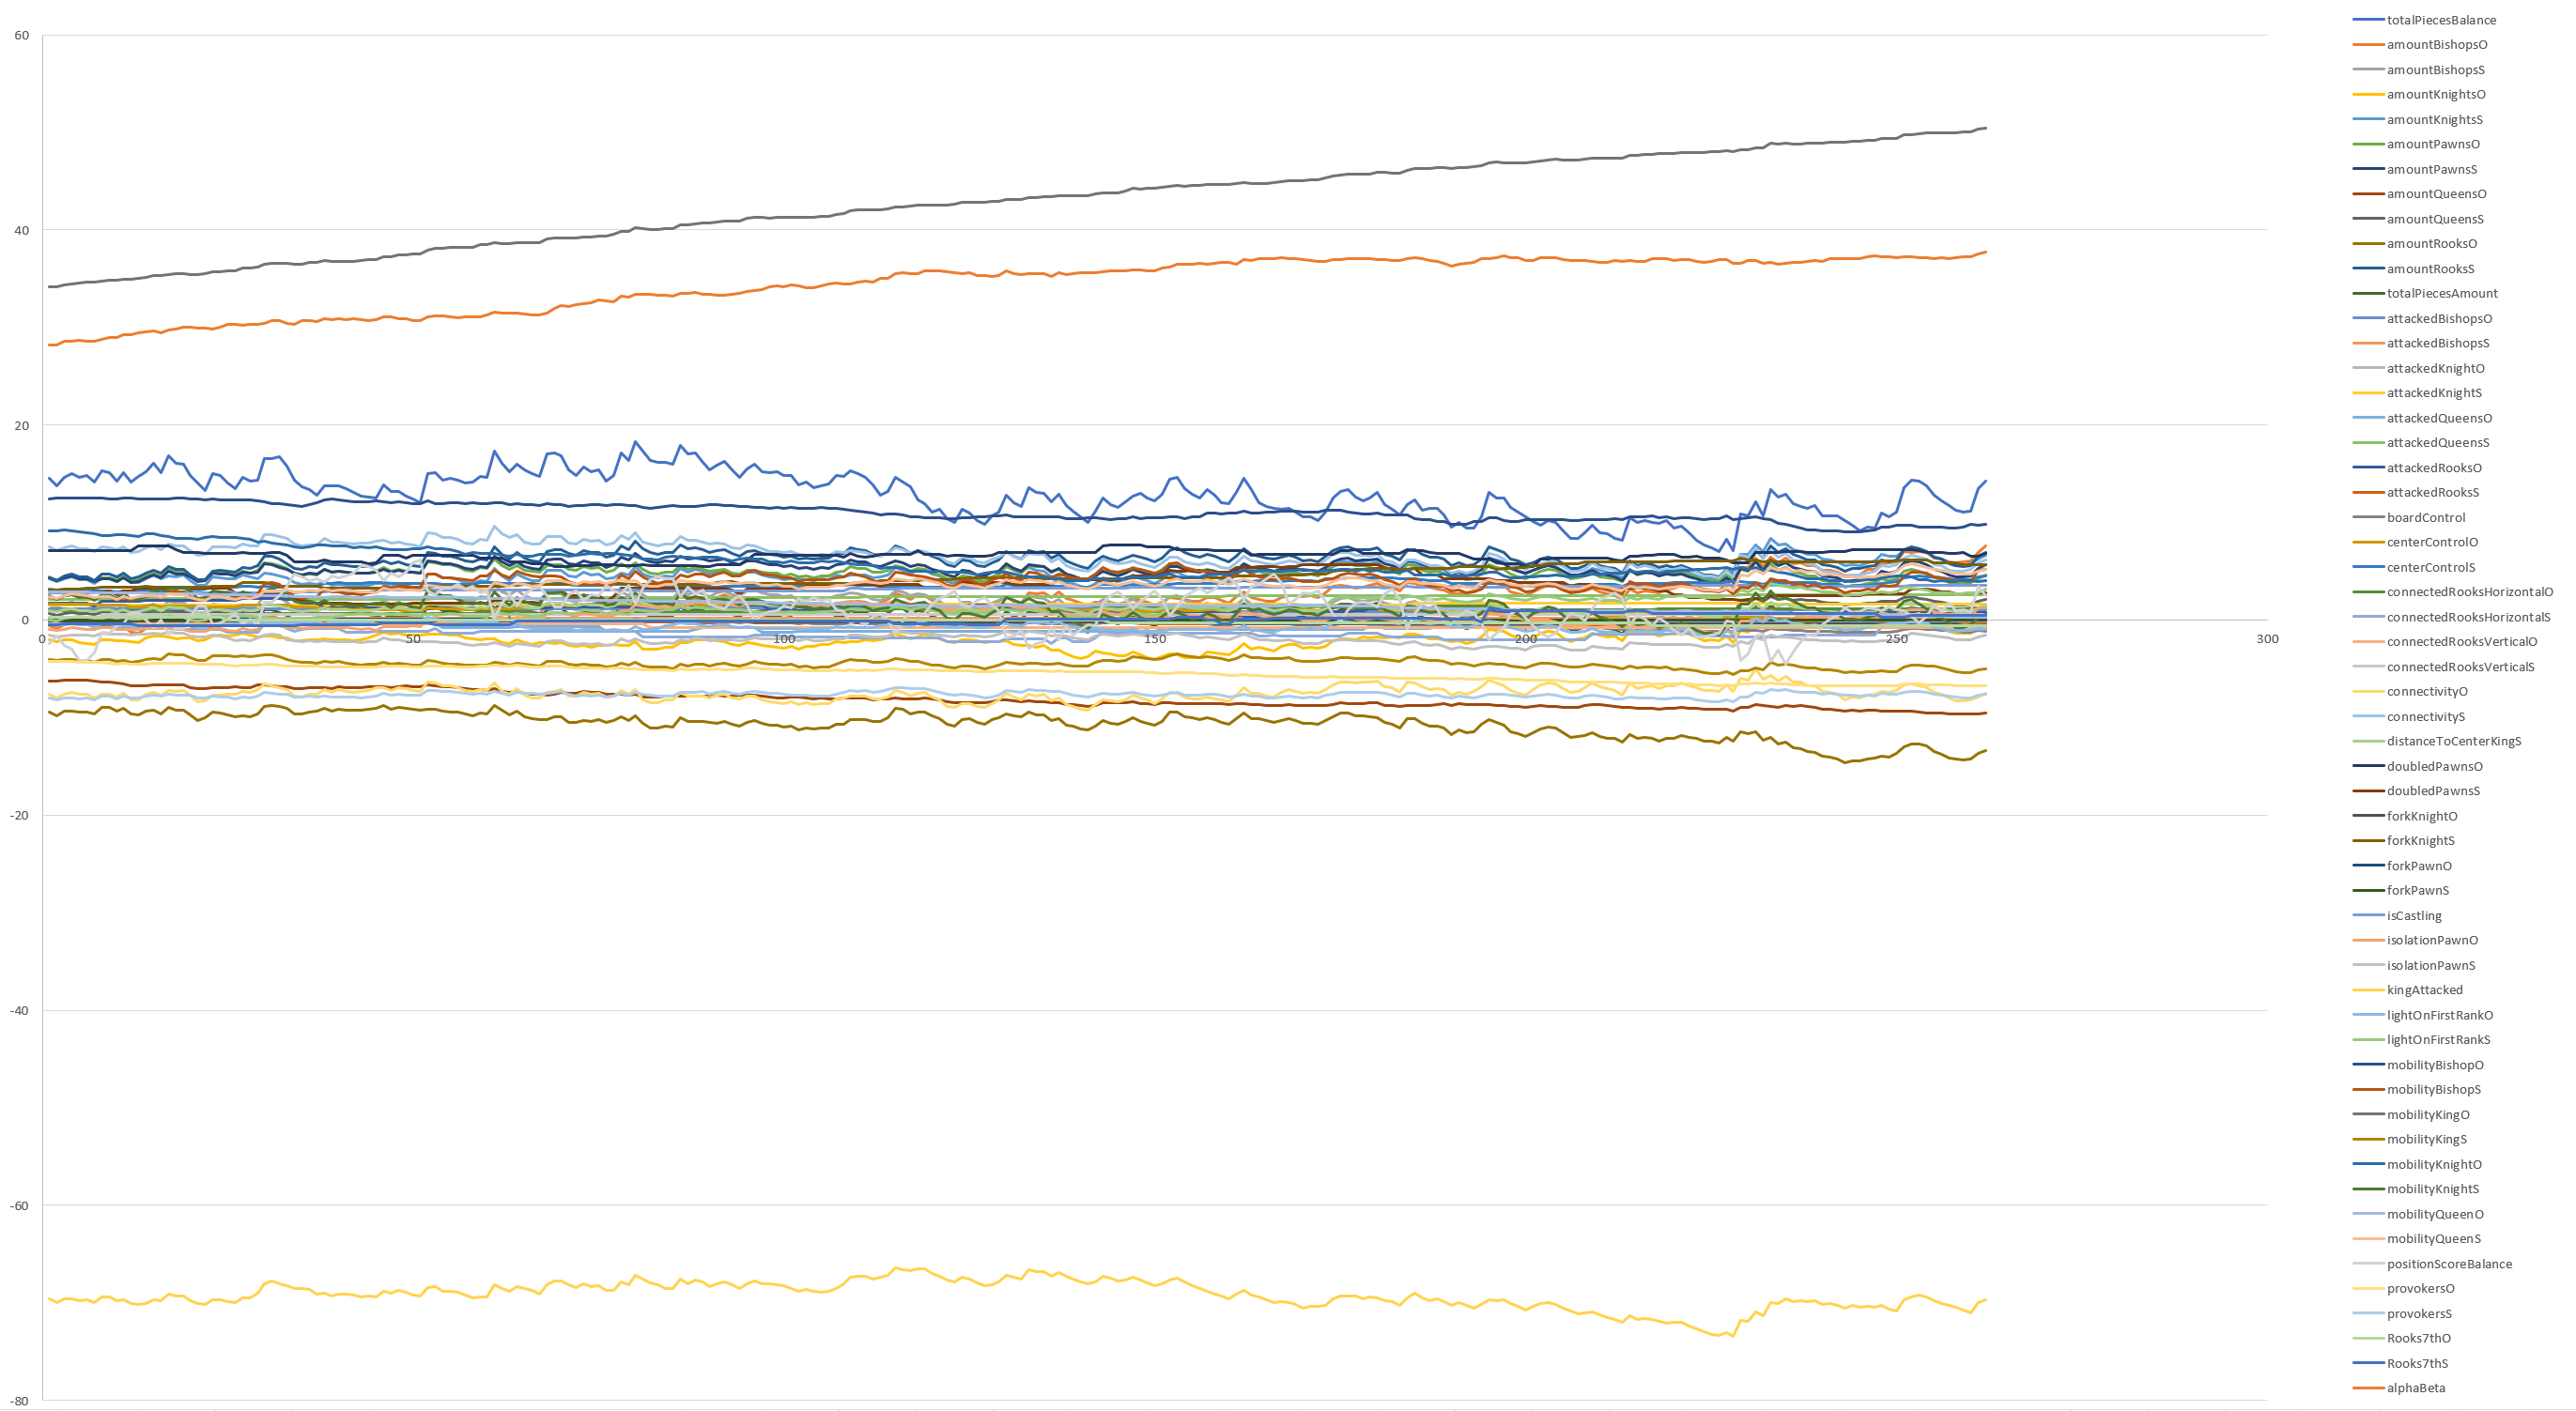
\includegraphics[width=\textwidth]{images/stockfish.png}
    \caption{Weight history vs. Stockfish}
    \label{fig:stockfish}
\end {figure}

Command:\\
\codeword{python3 train -o stockfish --skill 0 --depth 10 -tt 5 -dt 0 -e 0.3 -d 0.6 -l 0.01 -q -i -1}
\pagebreak

\section{GrandQ vs. Alpha-Beta (544 - 5732)}

Daarna hebben we nog 2 leersessies tegen onze alpha-beta agent laten spelen. De eerste leersessie was met dezelfde alpha en discount als tegen stockfish. Bij de 2 de leersessie hadden we deze verlaagd om de agent zich meer greedy te doen gedragen.

Onze agent wint $34\%$ van de spelletjes na volledig getrained te zijn, speelt gelijk voor $21\%$ van de spelletjes en $45\%$ van de tijd spelen onze agents een onbepaald spel. Deze staat is als de trainer het spel vroegtijdig stopt dit gebeurt na 130 zetten voor elke speler. Dit is om te voorkomen dat de agents zichzelf in een loop spelen en zo het trainen verschikkelijk doen vertragen.

\begin{figure}[h]
    \centering
    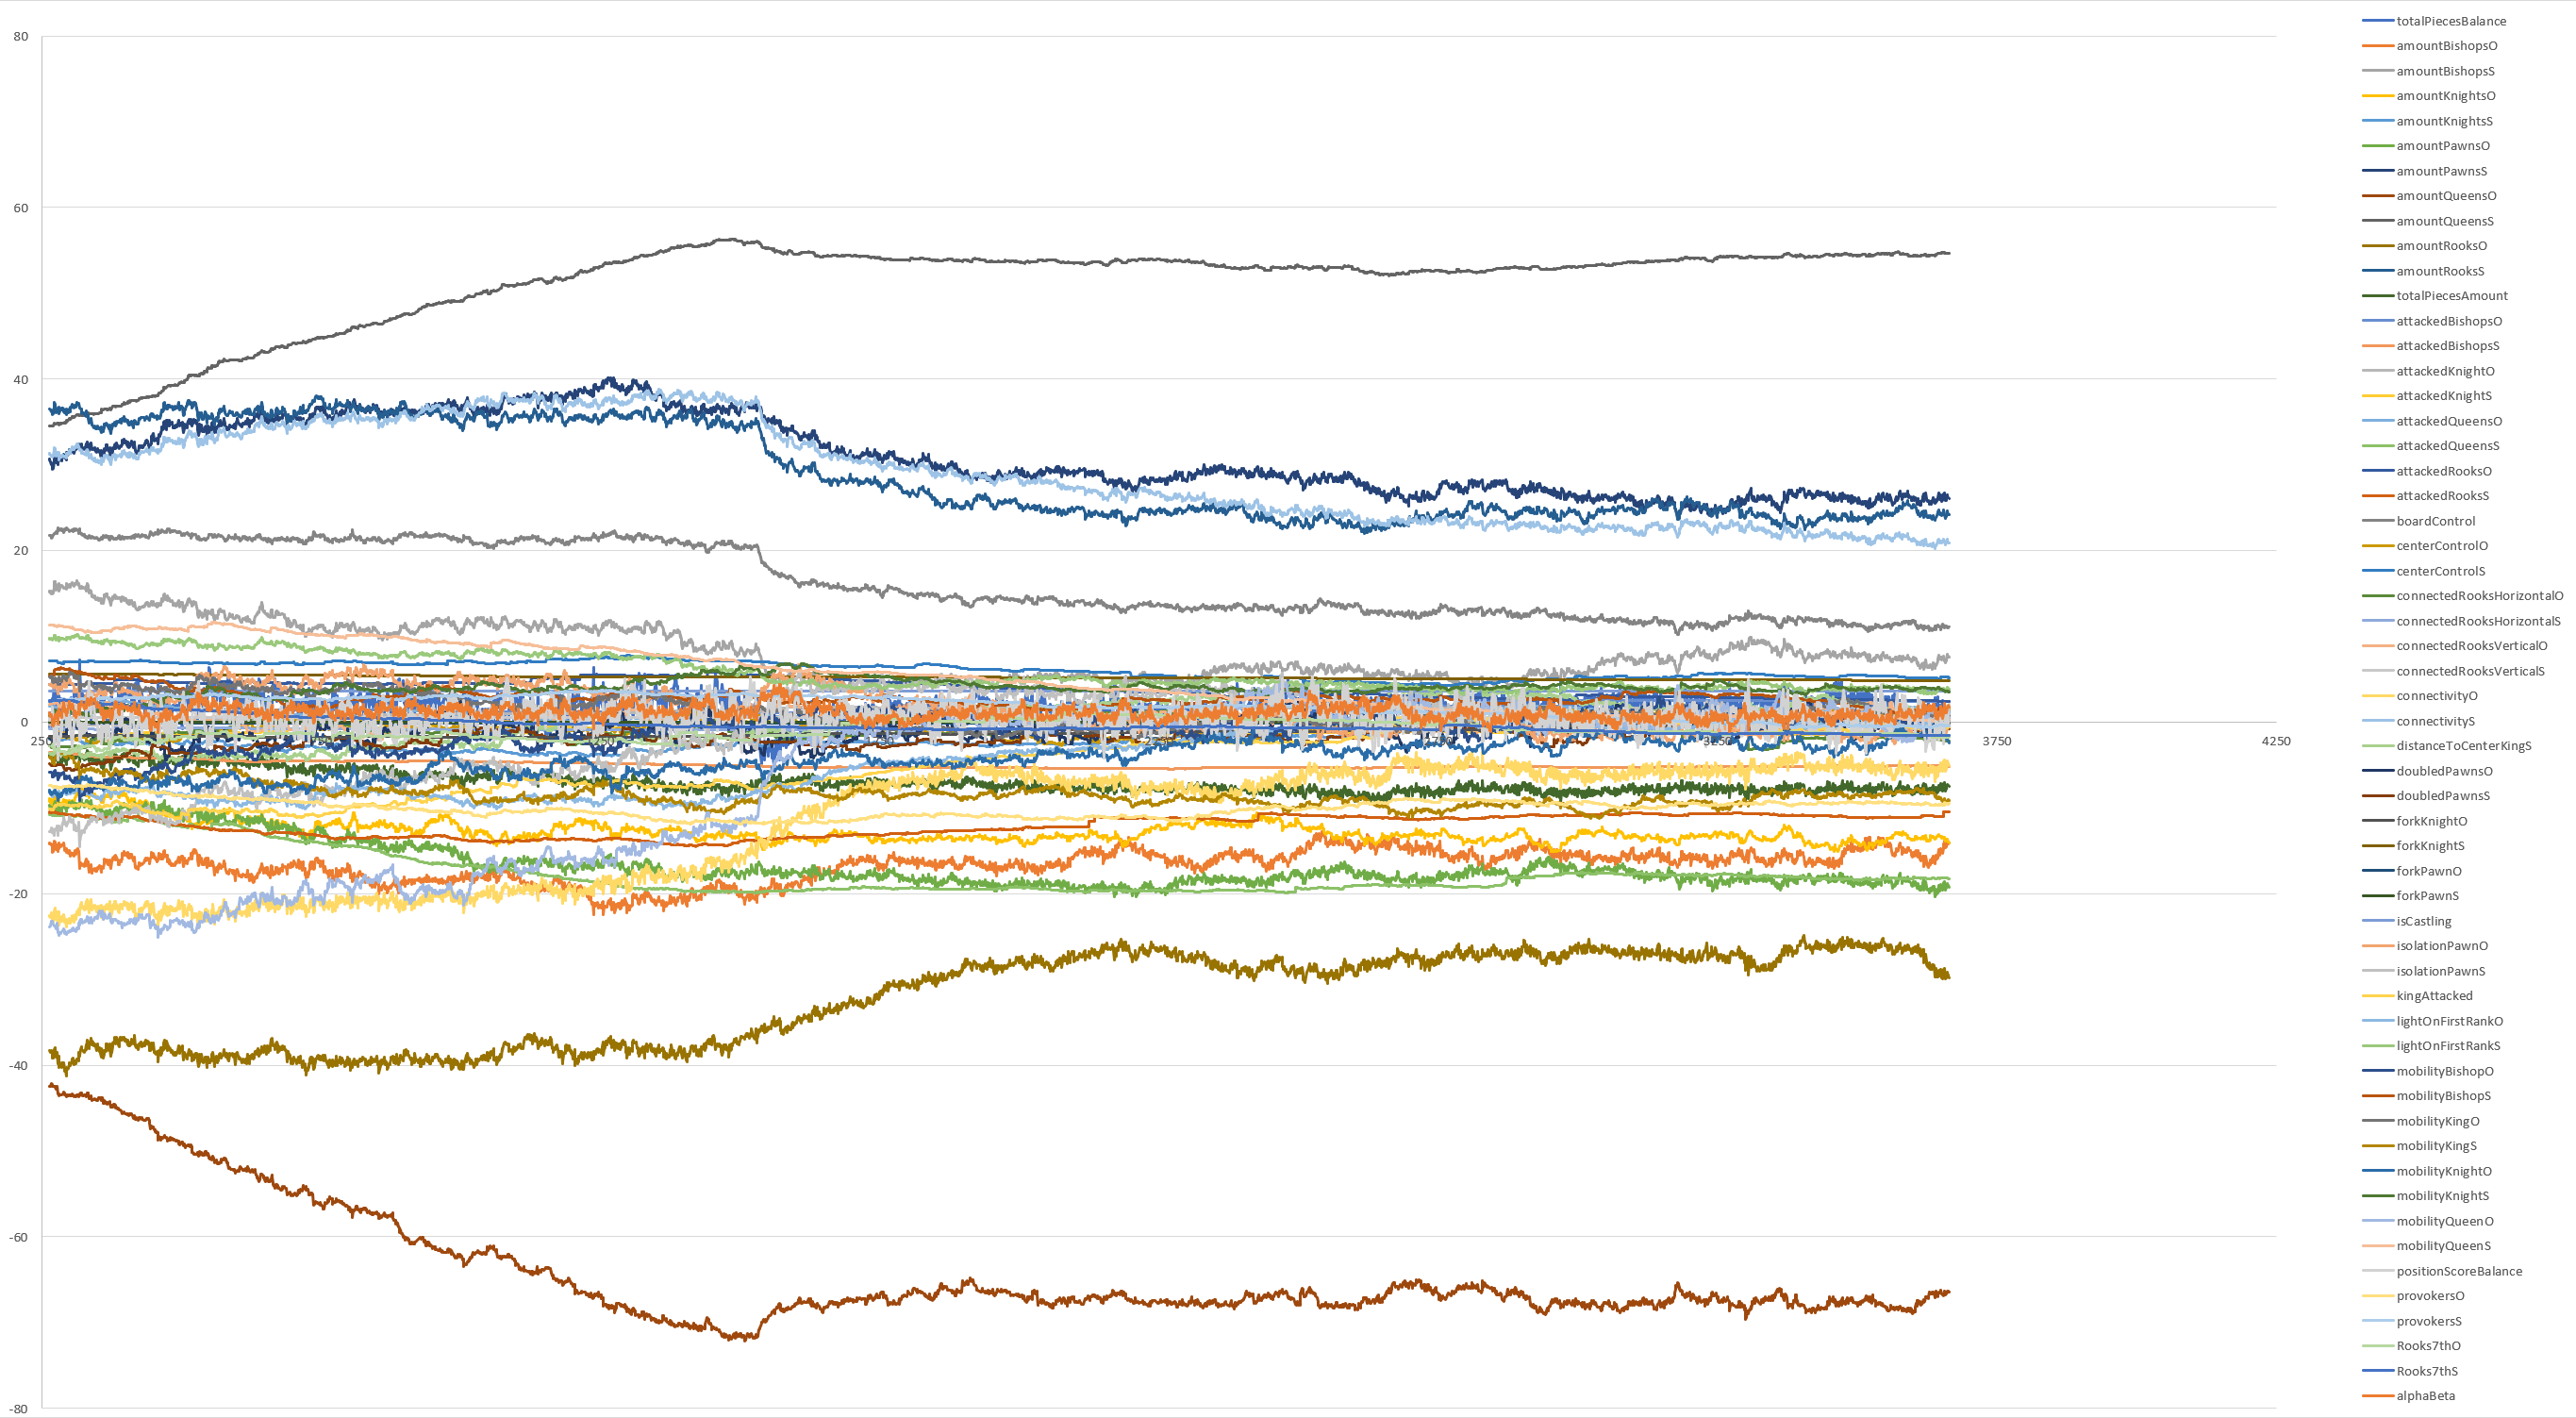
\includegraphics[width=\textwidth]{images/ab.png}
    \caption{Weight history vs. Alpha-Beta}
    \label{fig:ab}
\end {figure}

Command:\\
\codeword{python3 train -o ab --depth 10 -tt 5 -dt 0 -e 0.3 -d 0.6 -l 0.01 -q -i -1}

Command na ongveer 1500 episodes:\\
\codeword{python3 train -o ab --depth 10 -tt 5 -dt 0 -e 0.2 -d 0.4 -l 0.01 -q -i -1}

\section{Git Repository:}
Je kan onze code en ons getrained bestand ook terug vinden op gitlab: 
\begin{itemize}
    \item Repository: \href{https://gitlab.com/Artificiele_Intelligentie/chess}{\color{blue}\underline{https://gitlab.com/Artificiele\_Intelligentie/chess}}
    \item \href{https://gitlab.com/Artificiele_Intelligentie/chess/-/raw/master/grandQ.json}{\color{blue}\underline{Getraind bestand}}
\end{itemize}

\bibliography{sources}
\bibliographystyle{ieeetr}

\end{document}
